%%%%%%%%%%%%%%%%%%%%%%%%%%%%%%%%%%%%%%%%%%%%

\subsection{LocationChoice. Status: ready}

\subsubsection{{Maintenance and Questions}}

A. Horni, IVT (horni\_at\_IVT.baug.ethz.ch)

\subsubsection{{Javadoc}}

\href{http://www.matsim.org/javadoc/org/matsim/locationchoice/package-summary.html}{www.matsim.org/javadoc/org/matsim/locationchoice/package-summary.html}



%%\subsubsection{{\textbf{Config Parameters\hypertarget{parameters}{}}}}
\subsubsection{Config Parameters}


\href{http://www.matsim.org/javadoc/org/matsim/locationchoice/package-summary.html#locationchoice_parameters}{www.matsim.org/javadoc/org/matsim/locationchoice/package-summary.html\#locationchoice\_parameters}



\subsubsection{{Status}}

Ready

\subsubsection{{In Brief}}

MATSim provides destination choice based on three  different basic concepts. First, random search can be applied. Second,  local search implemented in the time geography framework is available  [1]. Third, the most recent module ist best response and includes random  error terms to make MATSim fully compatible with discrete choice theory  [2]. The authors recommend to use this recent module in general. Random  search should be utilized for algorithmic comparative investigations  only.

The time geography module provides the possibility to  take into account spatial competition in the activity location  infrastructure (see Fig.~\ref{fig:locachoice:3}). It is planned-after a thorough calibration-to integrate spatial competition in the best response version.

Estimation of a MATSim destination choice utility function for Switzerland is in development [3].
% EndFragment



\subsubsection{{Calling the Location Choice Strategy}}

The strategy module in the config file needs to be extended as follows:
\begin{lstlisting}{language=XML}
<module name="strategy">
    ...
    <param name="ModuleProbability_X" value="0.0 < double <=1.0" />
    <param name="Module_X" value="LocationChoice" />
    ...
</module>
\end{lstlisting}


\subsubsection{{I. Random Search}}

Due to slow convergence, this approach is only useful for very small scenarios.


\subsubsection{{II. Local Search With Time Geography}}

The MATSim local search destination choice module is  based on Hägerstrand's time geography. That is, in every replanning step  locations are chosen within the region restrained by travel time  budgets as defined by the time allocation module (see Fig.~\ref{fig:locachoice:1} and Fig.~\ref{fig:locachoice:2}). Within this region the choice is performed based on the MATSim utility function.

In more detail, the following procedure is  iteratively applied. An approximate choice set of locations is built to  begin with, where the constructing of this set is initially based on an  initial global travel speed assumption (\emph{recursionTravelSpeed}).  After tentatively choosing one location from this approximate set, the  actual accessibility in terms of travel time is checked. If the location  is not accessible it is rejected, the initial travel time is adapted  according to the \emph{recursionTravelSpeedChange}parameter  in the configuration file and a next trial is started. After a certain  number of failed trials to find an accessible location (\emph{maxRecursions}), the choice is made from the universal choice set.

The parameters \emph{recursionTravelSpeed}, \emph{recursionTravelSpeedChange}and \emph{maxRecursions }are explained in Section \hyperlink{parameters}{Parameters}


\subsubsection{{III. Best Response Including Random Error Terms}}

The parameters \emph{scaleEpsShopping }and \emph{scaleEpsLeisure }correspond to f$_Shopping$ and f$_Leisure$ in [2]. \emph{probChoiceSetSize }is $\Phi$, epsilonDistribution, \emph{tt\_}\emph{approximationLevel}, \emph{maxDistanceEpsilon}, and \emph{probChoiceExponent }are explained in in Section \hyperlink{parameters}{Parameters}.

The parameters \emph{scaleEpsShopping }and \emph{scaleEpsLeisure }can be calibrated, based on e.g., travel distance distributions as described in [2].

NOTE: This  variant will NOT work as described in Ref. [2] when configuring it as  described above. Additionally, the scoring function needs to be  modified. As of now, there does not seem to be a way to achieve  this without some Java programming. kai, jan'13

\subsubsection{{Spatial Competition: Facility Load Penalty Computation}}

Similar to route and time choice being influenced by  the competition in transport infrastructure it can be expected that  competition in activities infrastructure has an effect on destination  choice. Consequently, the utility of performing an activity is dependend  on the actual load of the activities infrastructure at least for some  activities such as e.g., grocery shopping (e.g.; searching for a parking  space or waiting time at cash points etc.). In MATSim spatial  competition is taken into account, which has shown to reduce the number  of implausibly overcrowded locations (see \hyperlink{Figure3}{Figure 3} below).

The score for perfoming an activity is calculated as follows:
\[
score = (1- fp) * score\_without\_penalty
\]
\[
fp = Max(0.5, fcrf)
\]
\[
fcrf = restraintFcnFactor * [(facility load) / (facility capacity)]^{restraintFcnExp}
\]
The parameters \emph{restraintFcnFactor}and \emph{restraintFcnExp }are explained in the section \hyperlink{parameters}{Parameters}


\subsubsection{{Literature}}

[1] Horni, A., D.M. Scott, M. Balmer and K.W. Axhausen (2009)  Location choice modeling for shopping and leisure activities with  MATSim: Combining micro-simulation and time geography, \emph{Transportation Research Record}, \textbf{2135}, 87-95.

[2] Horni, A., K. Nagel and K.W. Axhausen (2011) High-Resolution Destination Choice in Agent-Based Demand Models, \emph{Arbeitsberichte Verkehrs- und Raumplanung}, \textbf{682}, IVT, ETH Zürich, Zürich.

[3] Horni, A., D. Charypar and K.W. Axhausen (2011) Empirically  approaching destination choice set formation, paper presented at the \emph{90$^th$ Annual Meeting of the Transportation Research Board}, Washington, D.C., January 2011.

\subsubsection{Figures}

\begin{figure}[htp]
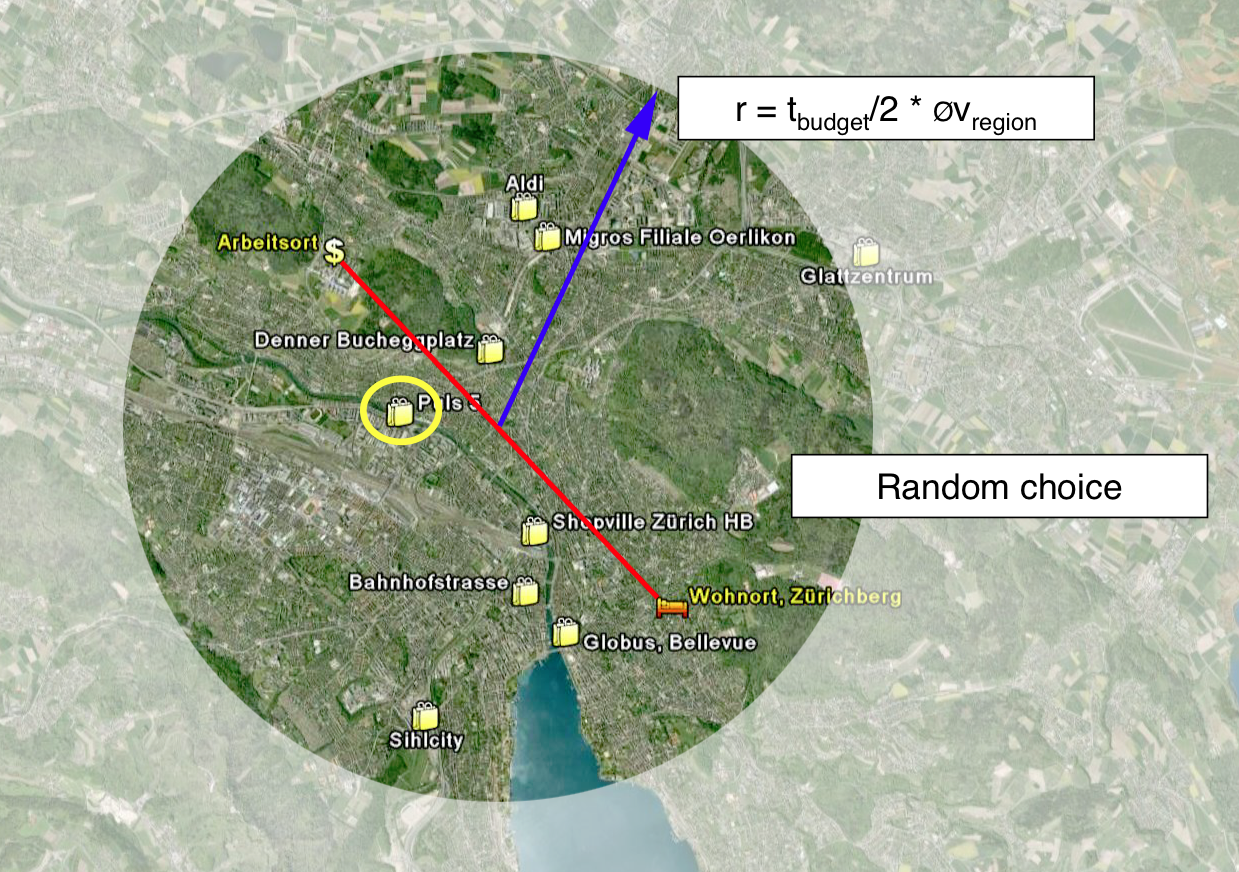
\includegraphics[width=.9\textwidth]{figures/locationChoice/locachoice1.png}
\caption{Region restrained by travel time budget}
\label{fig:locachoice:1}
\end{figure}

\begin{figure}[htp]
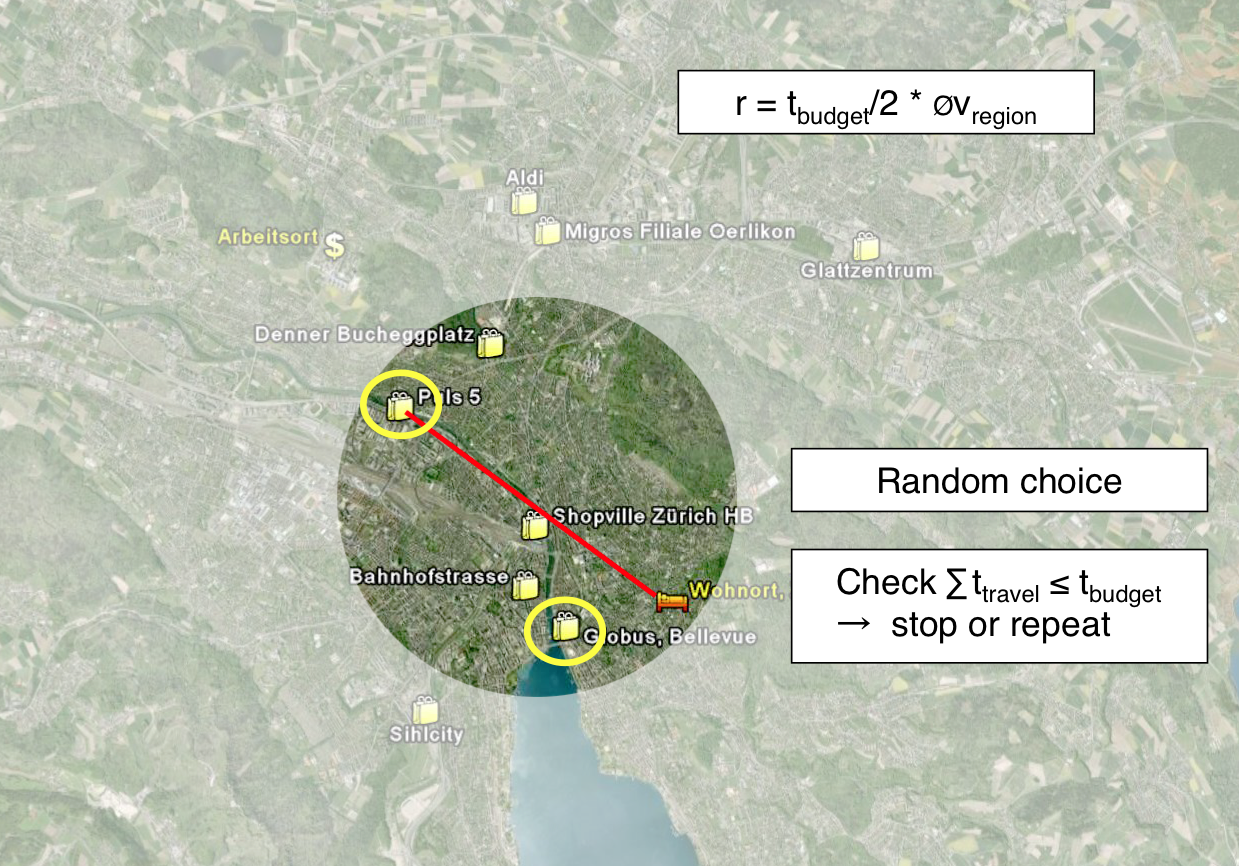
\includegraphics[width=.9\textwidth]{figures/locationChoice/locachoice2.png}
\caption{Region restrained by travel time budget}
\label{fig:locachoice:2}
\end{figure}

\begin{figure}[htp]
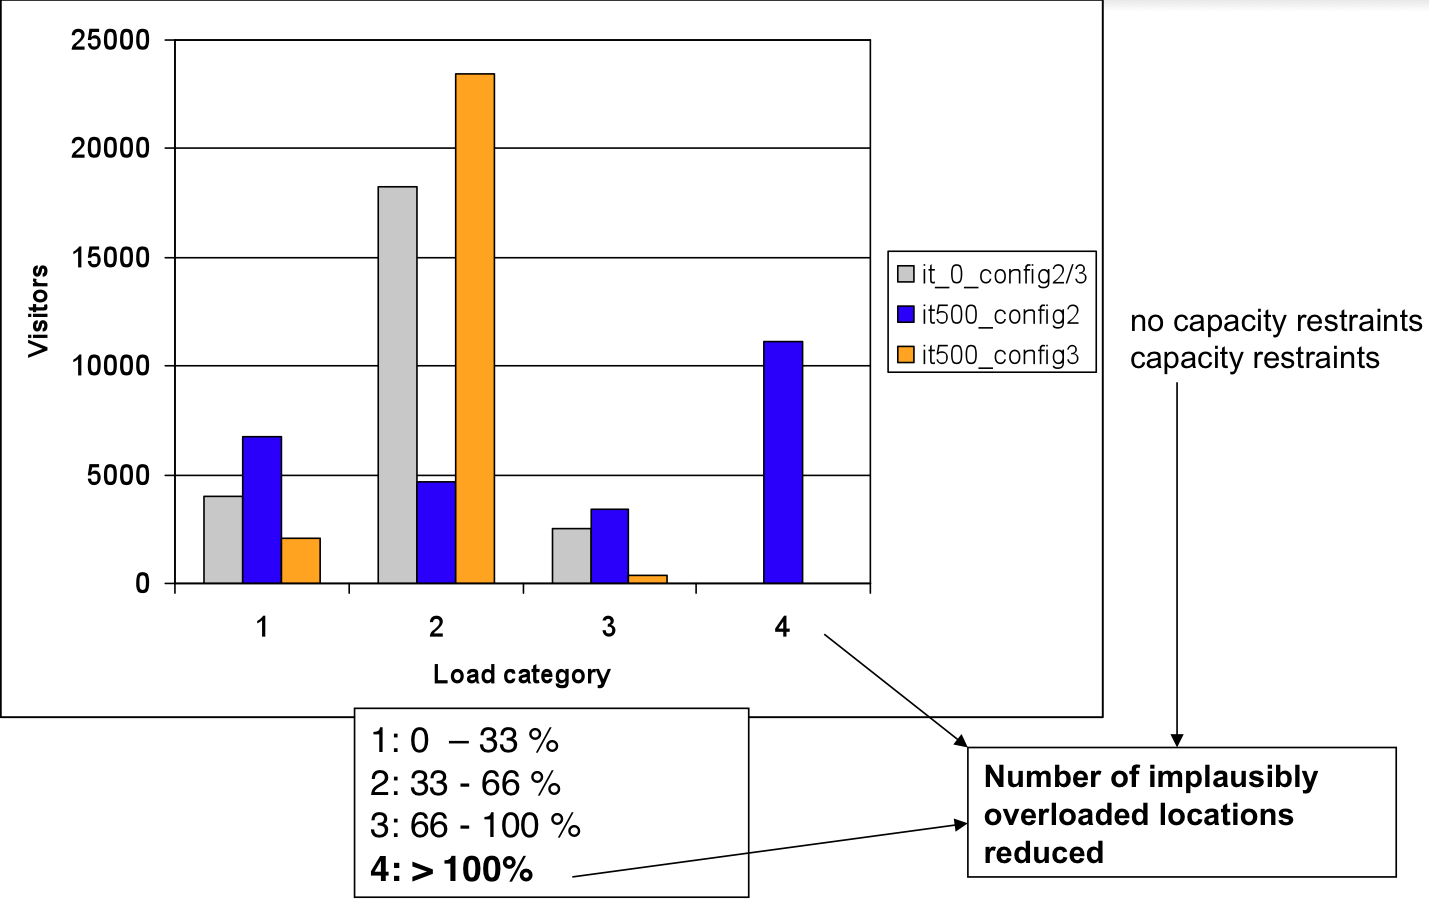
\includegraphics[width=.9\textwidth]{figures/locationChoice/locachoice_capacities.png}
\caption{Taking spatial competition into account}
\label{fig:locachoice:3}
\end{figure}




%%%%%%%%%%%%%%%%%%%%%%%%%%%%%%%%%%%%%%%%%%%%
